\documentclass{standalone}
\usepackage{tikz}

\usetikzlibrary{calc,math}

\newcommand{\nnormals}{8}


\begin{document}

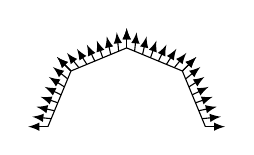
\begin{tikzpicture}
  \foreach[evaluate={\i*45} as \a,evaluate={(\i+1) * 45} as \b,evaluate={(\a+\b)/2} as \ab] \i in {0,...,3} {
    \coordinate (p) at (\a:1);
    \coordinate (q) at (\b:1);
    \draw (p) -- (q);

    \foreach[evaluate={(\j-1) / (\nnormals-1)} as \t] \j in {1,...,\nnormals} {
      \coordinate (r) at ($ (p) ! \t ! (q) $);
      \draw[-latex] (r) -- ($ (r) ! -.25 ! (0,0) $);
    }
  }
\end{tikzpicture}

\end{document}